\documentclass[a4paper,11pt]{article} 
\usepackage[english, french]{babel}
\usepackage[utf8]{inputenc}

\usepackage{graphicx}
\usepackage{fancyhdr}
\usepackage{lastpage}
\usepackage{amsmath}
\usepackage{xspace}
\usepackage{textcomp}

\usepackage{hyperref}

\usepackage[top=20mm, bottom=20mm, left=25mm, right=25mm]{geometry}

\pagestyle{fancy}

\usepackage{helvet}

\usepackage{verbatim}
\usepackage{amsmath}
\usepackage[table]{xcolor}
\definecolor{bleugris}{rgb}{.2,.4,.5}

\definecolor{colKeys}{rgb}{0,0,1} 
\definecolor{colIdentifier}{rgb}{0,0,0} 
\definecolor{colComments}{rgb}{0,0.5,1} 
\definecolor{colString}{rgb}{0.6,0.1,0.1} 

\usepackage{listings}
\lstset{%configuration de listings 
float=hbp,% 
basicstyle=\ttfamily\small, % 
identifierstyle=\color{colIdentifier}, % 
keywordstyle=\color{colKeys}, % 
stringstyle=\color{colString}, % 
commentstyle=\color{colComments}, % 
columns=flexible, % 
tabsize=2, % 
frame=trBL, % 
frameround=tttt, % 
extendedchars=true, % 
showspaces=false, % 
showstringspaces=false, % 
numbers=left, % 
numberstyle=\tiny, % 
breaklines=true, % 
breakautoindent=true, % 
captionpos=b,% 
xrightmargin=-1cm, % 
xleftmargin=-1cm 
} 
\lstset{language=octave} 
\lstset{commentstyle=\textit}

\newcommand{\nTitle}[1]{%
	\newpage 			%
	\vspace*{\fill}		%
	\begin{center}	%
		\part{#1}		%
	\end{center}
	\vspace*{\fill}		%
	\newpage			%
}

\newenvironment{nAbstract} 		%
{ 								%
	\newpage 					% 
	\vspace*{\fill}				%
	\begin{center}			 	%
		\begin{abstract}		%
}{								%
		\end{abstract}			%
	\end{center}				%
	\vspace*{\fill}				%
	\newpage					%
}


\newcommand{\nClass}[1]{{\color{bleugris}{\textsl{\textbf{#1}}}}}
\newcommand{\nParameter}[1]{{\color{gray}{\textbf{#1}}}}
\newcommand{\nMethod}[1]{{\color{gray}{\textbf{#1}}}}
\newcommand{\nConstant}[1]{\texttt{\uppercase{#1}}}
\newcommand{\nKeyword}[1]{\textsl{\textbf{#1}}}

 
%opening
\title{\textbf{Projet d'aide à la décision}}
\author{Paul \textsc{Adenot}, Etienne \textsc{Brodu}, Maxime \textsc{Gaudin},\\
Monica \textsc{Golumbeanu}, Nor \textsc{El Malki}, Yoann \textsc{Rodière}}
\lhead{Hexanome 4203}
\cfoot{\thepage\ de \pageref{LastPage}}

\begin{document}
\maketitle
{ \footnotesize % pour être sur qu'il tient sur une page
\tableofcontents
}

\begin{nAbstract}
L'objet de ce rapport est de présenter une solution capable de trouver une
stratégie de production, menant à un contentement optimal des différent
acteurs :
\begin{itemize}
  \item Le comptable
  \item Le responsable des ateliers
  \item Le responsable des stocks
  \item Le responsable commercial
\end{itemize}
~\\
La démarche sera quant à elle incrémenta le puisque nous fournirons dans un
premier temps des optimum très locaux, respectant un nombre limités de
contraintes et de critères, puis nous combinerons ces différents résultat afin
de converger vers une solution prenant en compte l'intérêt de chacun.
\end{nAbstract}

\nTitle{Programmation Linéaire monocritère}

\section{Données}
Soient :
\begin{itemize}
  \item \textbf{T} la matrice des temps unitaires d'usinage d'un produit sur une
  machine (minutes) (\textsl{C.f. Table 1}).
  \item \textbf{Q} la matrice de quantité de matières premières par produit
  (\textsl{C.f. Table 2}).
  \item \textbf{S} la matrice des quantité maximum de matières premières
  (\textsl{C.f. Table 3}).
  \item \textbf{V} la matrice des prix de vente des produits finis (\textsl{C.f.
  Table 4})
  \item \textbf{A} la matrice des prix d'achat des matières premières.
  \item \textbf{C} la matrice des coûts horaires des machines (\textsl{C.f.
  Table 5}).
\end{itemize}

\subsection{Contraintes}
Considérons :
\begin{itemize}
  \item 7 machines $j \in {1, 2, 3, 4, 5, 6 ,7}$
  \item 6 produits $i \in {A, B, C, D, E, F}$
  \item $n_i$ le nombre de d'unités $i$ fabriquées
\end{itemize}
~\\
L'ensemble de la chaine de production est régie par les contraintes suivantes
:\\
\begin{itemize}
  \item \textbf{Le nombre de produits usinés :} Il doit être non nul
  \begin{equation} 
  	\forall i, n_i \ge 0 \label{C0}
  \end{equation}
  
  \item \textbf{La quantité de matières premières :} Elle doit
  être positive.
  \begin{equation} 
  	\forall i, S_i \ge 0 \label{C0}
  \end{equation}
  
  \item \textbf{Le temps d'occupation de chaque machine $i$:} Il doit être
  inférieur au temps de travail
  \begin{equation} 
  	\sum_{j = A}^{F} T_{j,i} . n_j \leq 2.8.60.5 = 4800 \label{C1}
  \end{equation} 
  soit un temps de travail en deux huit, 5 jours par semaine.
  
  \item \textbf{L'utilisation de chaque matière première  $i$:} Elle doit être
  inférieure au stock
  \begin{equation} 
  	\sum_{j = A}^{F} Q_{i,j} . n_j \leq S_i \label{C2}
  \end{equation} 
\end{itemize}

\section{Objectif : Comptable}
Le comptable cherche à maximiser les bénefices sous les contraintes définies
précedemment.

\subsection{Modélisation}
Soit $n_i$ le nombre de produit $i$ fabriqué. Le coup fixe de production
n'influant pas sur notre décision, nous ne considérerons que le coût variable de
production. Il est défini par la formule suivante:
\begin{displaymath}
CV(i) = n_i * \left (\sum_{j = 1}^{7} T_{i,j} .
\frac{C_{i,j}}{60} + \sum_{k = 1}^{3} Q_{k,i} . A_{k} \right )
\end{displaymath}
~\\
Le chiffre d'affaire par produit est :
\begin{displaymath}
CA(i) = n_i . V_i
\end{displaymath}
~\\
Par conséquent le bénefice par produit se calcule de la manière suivante :
\begin{eqnarray*}
	B(i) &=& CA(i) - CV(i)\\
	B(i) &=& n_i * \left (V_i - \sum_{j = 1}^{7} T_{i,j} . \frac{C_{i,j}}{60} +
	\sum_{k = 1}^{3} Q_{k,i} . A_{k} \right )
\end{eqnarray*}
\newpage
\section{Objectif : Responsable d'atelier}
Le responsable d'atelier cherche à maximiser le nombre d'unités (toutes
catégories confondues) produites sous les contraintes définies précedemment.

\subsection{Modélisation}
Soit $N$ le nombre de produits fabriqués.

\begin{equation}
	N = \sum_{i = A}^{F}
\end{equation} 
\newpage
\section{Stratégie du point de vue du \textsl{Responsable des stocks}}
\label{sec:stocks}

Le responsable des stocks cherche à minimiser la contenance du stock,
\textsl{i.e.} le nombre de produits entreposés ajouté à la quantité de
matières premières. Aucune contrainte particulière n'est ajoutée mais la
recherche de l'optimum se fait sous les contraintes définies précédemment.

\subsection{Modélisation}
Soit $Stock(n_{i})$ le nombre d'unités de stock nécessaires pour stocker les
produits fabriqués et les matières premières nécessaires.\\
Cette fonction est évidemment la somme des produits fabriqués et de la quantité de matières
premières nécessaire à leur fabrication.\\
~\\
Supposons qu'\textbf{un produit fabriqué correspond à une unité de stock.}\\
~\\
Ainsi, soient :
\begin{itemize}
	\item $n_{i}$ la quantité de produits usinés (pour chaque produit $i$)
	\item $Q_{j,i}$ la quantité de matière première par produit pour chaque produit $i$ et chaque matière première $j$.
\end{itemize}
~\\
Alors :
\begin{equation}
	Stock(n) = \sum_{i} (n_{i} + n_{i} \times \sum_{j} Q_{j,i})
\end{equation}

La représentation matricielle de cette fonction sera alors :

\begin{equation}
	M_S = \begin{pmatrix}
		1 & 1 & 1 & 1 & 1 & 1
	\end{pmatrix} + (
	\begin{pmatrix}
		1 & 1 & 1
	\end{pmatrix}
	\times Q)
\end{equation}

\subsection{Stratégie adoptée}
Un résultat trivial est de ne fabriquer aucun produit :
\begin{equation}
    \begin{pmatrix}
	0 \\ 0 \\ 0 \\ 0 \\ 0 \\ 0
    \end{pmatrix}
\end{equation}

En effet, en l'absence de production, aucun stock n'est nécessaire. Ce résultat
n'est pas satisfaisant.\\
Nous allons donc nous intéresser à un second critère : \textbf{les bénéfices de l'entreprise}.\\
Pour ce faire, nous allons nous utiliser les résultats obtenus en imposant un minimum de bénéfices.\\
En réalisant les calculs sur plusieurs échelons, nous obtenons un résultat linéaire par morceaux. Le
raisonnement adopté est similaire à celui développé dans la section \ref{sec:monocrit}.

\begin{figure}[!ht]
	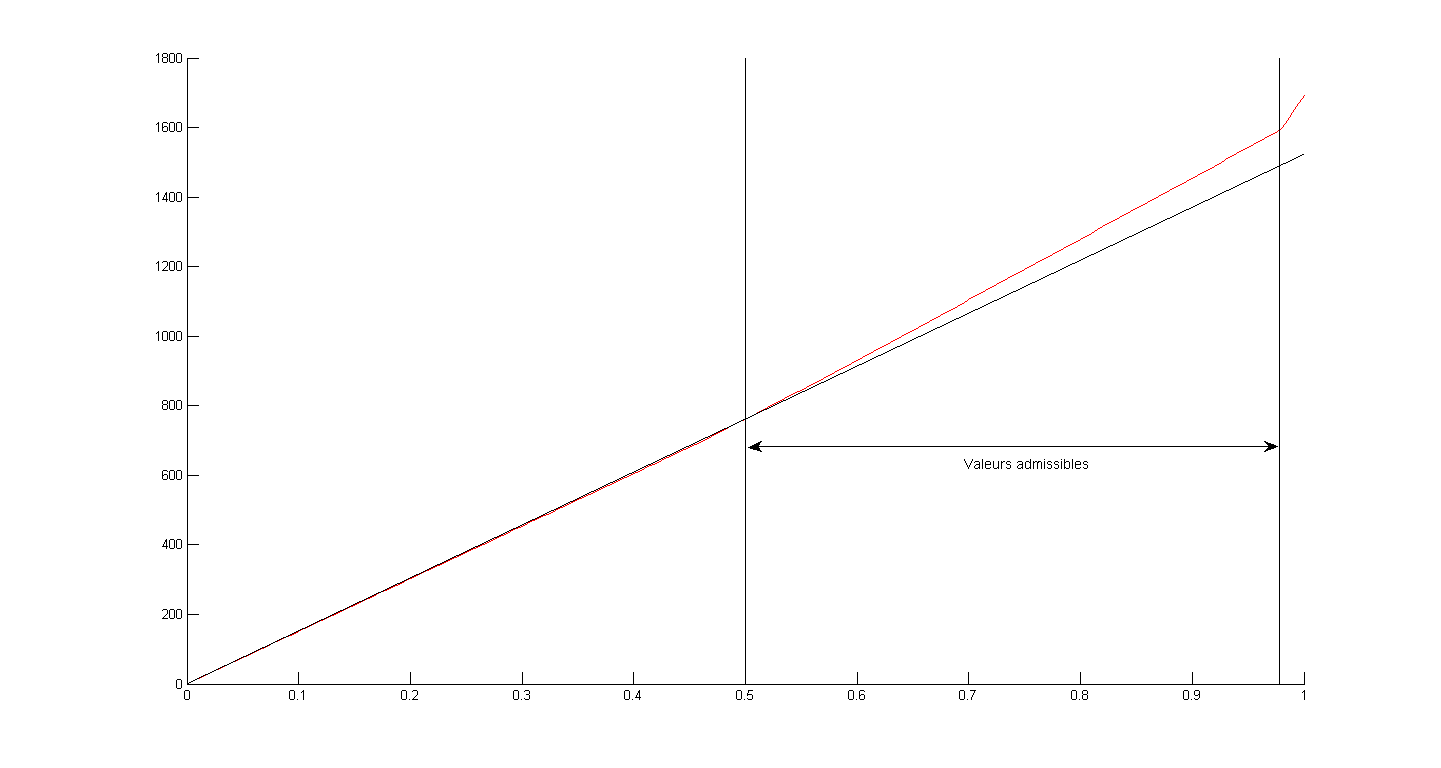
\includegraphics[width=\textwidth]{graphe_resp_stocks.png}
	\caption{Graphe de l'évolution des stocks en fonction du bénéfice}
\end{figure}

\subsubsection{Interprétation} 
De nombreuses valeurs sont équivalentes mathématiquement parlant et ne peuvent pas vraiment être départagées. 
Les choix possibles se situent dans la deuxième partie de la courbe :
\begin{itemize}
	\item En dessous, les bénéfices sont trop bas.
	\item Au dessus, les besoins de stockage augmentent beaucoup plus que les bénéfices. Nous perdons alors de vu notre
	objectif initial, \textsl{i.e.} avoir le moins de stock possible.
\end{itemize}

Nous obtenons donc une valeur comprise entre 50\% et 98\% de bénéfices. 
Pour 75\% du bénéfice maximum, nous obtenons le nombre de produits suivants :

\begin{equation}
\begin{pmatrix}
1,91903382074088 \times 10^{-10} \\
2,63753463514149 \times 10^{-10} \\ 
1,89174897968769 \times 10^{-10} \\
1,23691279441118 \times 10^{-10} \\ 
124,634235411818 \\
142,146305832495 
\end{pmatrix}
\end{equation}

\begin{center}
	\fbox{\textbf{Soit une quantité d'unités en stock de 1191,75640039347.}}
\end{center}
~\\
Cette étude de cas nous rappelle les limite d'une stratégie basée sur l'analyse d'un seul critère. En effet, 
en l'absence de contraintes assez fortes, le problème devient \og indécidable\fg mathématiquement.

C'est pourquoi nous allons combiner les 4 études réalisées pour affiner nos stratégies et obtenir une solution : 
\begin{itemize}
	\item Mathématiquement claire
	\item Respectant un ensemble de contraintes plus grand, et par conséquent qui se concentre plus sur les
	contraintes propres à l'entreprise \textbf{Optim}.
\end{itemize}

\newpage
\section{Objectif : Responsable commercial}
Le responsable commercial cherche à équilibrer le nombre
d'unités de ${A, B, C}$ (famille 1) et ${D, E, F}$ (famille 2) afin que ces deux
familles contiennent le même nombre d'unités ( à $\epsilon$
unité(s) près).\\
Autrement dit, l'écart entre le nombre d'unités produite pour la famille A et la famille B doit être inférieur à un seuil $\epsilon$.

\subsection{Modélisation}
Soient :
\begin{itemize}
  \item $N_1$ le nombre de produits de la famille 1 fabriqués.
  \item $N_2$ le nombre de produits de la famille 2 fabriqués.
\end{itemize}

\begin{eqnarray*}
	|N_1 - N_2| &\leq& \epsilon\\
	\Leftrightarrow -\epsilon \leq N_1 - N_2 &\leq& \epsilon\\
	\Leftrightarrow -\epsilon \leq \sum_{i = A}^{C} n_i - \sum_{j = D}^{F} n_j
	&\leq& \epsilon\\
\end{eqnarray*} 
Par concéquent, c'est cette nouvelle contrainte qui, venant s'ajouter aux
contraintes précédentes, va permettre de calculer le nombre d'unités A, B, C,
D, E, et F à fabriquer afin d'équilibrer les deux familles.\\
~\\
Nous obtenons la matrice suivante :
\begin{displaymath}
M = \left(
\begin{array}{cccccc}
1 & 1 & 1 & 1 & 1 & 1\\
\end{array}
\right)
\end{displaymath}
La matrice, très simple, représente la somme des différents produits.\\
La matrice des contraintes devient quant à elle :
INSÉRER MATRICE A MODIFIEE

\subsection{Décisions}

\subsection{Interprétation}
Evidemment, toutes les solutions triviales du type :
\begin{displaymath}
M_p = \left(
\begin{array}{cccccc}
N \pm \epsilon & N \pm \epsilon & N \pm \epsilon & N & N & N\\
\end{array}
\right)
\end{displaymath}
ou encore 
\begin{displaymath}
M_p = \left(
\begin{array}{cccccc}
N & N & N & N \pm \epsilon & N \pm \epsilon & N \pm \epsilon\\
\end{array}
\right)
\end{displaymath}
\begin{center}
\textsl{Où $M_p$ est la matrice du nombre de produit, et $N \in \mathbbm{N}$}
\end{center}
sont des solutions \emph{valables}.\\
~\\
Ceci met en évidence qu'avec les critères définis plus haut, il n'y a pas de
solution plus \og valable\fg ~qu'une autre. Par concéquent nous pouvons :
\begin{itemize}
  \item Choisir une solution au hasard
  \item Augmenter le nombre de critère et notamment ceux en rapport avec les
  stocks disponibles, le prix des matières premières, ou encore le temps
  d'usinage nécessaire.
\end{itemize}

~\newpage
\nTitle{Programmation linéaire multicritère}

\section{Objectifs}
L'objectif est de trouver une solution de compromis entre les différents responsables.
Pour trouver une telle solution nous serons amenés à utiliser la programmation multicritère (\emph{PLM}).
Auparavant, dans la partie 1, nous avons trouvé un optimum pour chaque
responsable indépendam\-ment, ce qui nous conduit à un point de mire. Dans un
monde parfait, ce point de mire respecterait les contraintes de chaque
responsable. Nous devons donc voir si tel est le cas. 

\section{Recherche du point de départ}
Si le point de mire est assez proche de l'ensemble des solutions acceptables,
nous choisirons une solution proche de celle d'un responsable.

Sinon, nous allons calculer la satisfaction de chaque objectif, sachant qu'une
solution a été retenue. Nous devrons alors définir des métriques, correspondant
à cette satisfaction. Par exemple, pour le comptable, cette satisfaction sera
exprimée par le ratio du bénéfice obtenue dans un solution par rapport au
bénéfice maximal.
Ensuite, nous choisirons comme point de départ la solution qui offre le plus de
satisfaction à tout le monde, par exemple en utilisant une moyenne pondérée,
dont la pondération sera basée sur \emph{l'importance} de chaque critère.

\section{Affinement de la solution}
La solution trouvée précédemment peut sûrement être optimisée. Il peut être
intéressant de perdre dans un critère, si cela nous fait gagner beaucoup dans
un autre critère, d'autant plus si ce second critère est jugé plus
\emph{intéressant} que le premier.

\section{Métriques utilisées}
Cette section décrit les métriques utilisées pour caractériser une solution, du
point de vue d'un cadre de l'entreprise. Les solutions pourront ainsi être
comparées entre elles.

\paragraph{Comptable :}
La métrique utilisée sera le pourcentage du bénéfice par rapport au bénéfice
maximum :
$$
M_{Comptable} = \frac{B_{S}}{B_{max}} \times 100
$$

\paragraph{Responsable d'atelier}
La métrique utilisée sera le pourcentage du nombre de produits fabriqués par
rapport au nombre maximum :
$$
M_{Atelier} = \frac{N_{S}}{N_{max}} \times 100
$$

\paragraph{Responsable des stocks}
Pour élaborer la métrique de satisfaction pour le responsable des stocks nous
opterons pour la fonction suivante, qui correspond à ce qui était précédemment
annoncé dans la partie 1 (page \pageref{stocks}).

\begin{figure}[!ht]
\begin{center}
    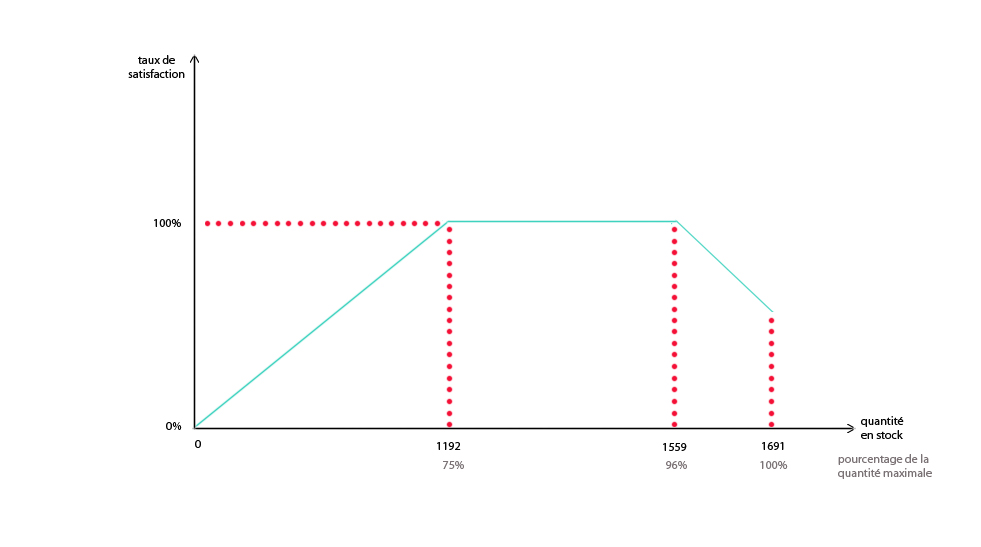
\includegraphics[width=\linewidth]{multicritere_graphe_stocks.png}
    \caption{Représentation graphique de la métrique pour le responsable des
	stocks.}
	\end{center}
\end{figure}

Cette fonction est décrite par l'expression suivante :
$$
M_{Stocks} = \left\{ 
    \begin{array}{l l l}
	\frac{x}{1192} \text{ si } x \in \text{[0 ; 1192]} \\
	x=1 \text{ si } x \in [1192 ; 1559]\\
	\frac{-x}{1192}+ 1+\frac{1559}{1192} \text{ si } x \in \text{[1559 ;
	    1691]}\\
    \end{array}
\right.
$$

Cette fonction pourrait être justifiée par le fait que plus on s’éloigne des
valeurs admises moins le responsable des stocks est satisfait.


\paragraph{Responsable commercial}
La métrique utilisée sera l'écart par rapport à un équilibre parfait.
Si autant de produit de la famille de produit 1 (comprenant les produits A, B
et C) que de la famille 2 (comprenant les produits D, E et F), la métrique sera
à 100\%.
Si une seule famille de produit est fabriquée, la métrique devra valoir zéro.

Si $F_1$ (respectivement $F_2$ est le nombre de produit de la famille 1
(respectivement famille 2), la métrique sera :
$$
M_{Commercial} = \left( 1 - \frac{|F_1 - F_2|}{F_1 + F_2} \right) \times 100
$$

\section{Utilisation}
Les résultats seront placés dans un tableau de ce type, qui qui permettra d'un
seul coup d'œil de voir la meilleur des solutions.
La colonne en rouge se lira par exemple : 
\begin{center}
«~En suivant la volonté du responsable d'atelier, le comptable aura une
satisfaction de $96.5498\%$~»
\end{center}

    \begin{center}
	\begin{tabular}{|l|c|c|c|c|}
	    \hline
	    \cellcolor[gray]{0.9} & Comptable& Atelier & Stock & Commercial  \\
	    \hline
	    Comptable & 100.000\% & 94.7678\% & 88.9030\% & 11.4302\% \\
	    \hline
	    Atelier   & \cellcolor{red}96.5498\% & 100.000\% & 77.7846\% & 50.6491\% \\
	    \hline
	    Stock     & 74.1546\% & 70.8003\% & 99.9796\% & 0.00000\% \\
	    \hline
	    Commercial& 81.8653\% & 93.4330\% & 80.2626\% & 100.000\% \\
	    \hline
	\end{tabular}
    \end{center}

On voit déjà que la solution du commercial contente, dans une certaine mesure,
l'ensemble des responsables de l'entreprise, toutes les métriques sont
supérieures à 80\%.

\section{Optimisation}
Nous allons dans cette partie essayer de modifier les solutions précédentes
pour trouver une solution qui tente de maximiser la satisfaction des différents
responsables.

Le but premier d'une entreprise étant de faire du profit, et les meilleur 
manière de faire du profit étant souvent maximiser le bénéfice et d'avoir une
bonne politique commerciale, nous allons donc favoriser ces critère (bénéfice et
équilibrage des solutions), en leur appliquant un léger coefficient.

Nous allons par la même regarder l'évolution des autres critères lorsque ce
coefficient évolue, c'est à dire recalculer les différentes métriques.

Il apparaît plausible qu'avoir un \emph{stock non optimal} peut être acceptable
si c'est pour avoir un bénéfice plus important, dans une certaine mesure. Une
dégradation de la satisfaction du responsable des stock sera donc moins
pénalisante, en terme de qualité de solution, qu'une baisse dans la satisfaction
du commercial (produire sans vendre ne sert pas à grand chose, en terme de
rentabilité).

De la même manière, produire un nombre de produit important peut être
intéressant, mais cela ne doit pas aller à l'encontre du profit et de la
mauvaise répartition de la production.

Nous pouvons donc donner des coefficients aux critères :

\begin{table}[h!]
\begin{center}
\begin{tabular}{|l||c|c|c|c|}
\hline
    Responsable & Comptable & Atelier &  Stocks & Commercial  \\
	\hline
    Coefficient & 1.2	    & 0.8     & 0.8	& 1.2 \\
	\hline
	\end{tabular}
	\end{center}
\caption{Coefficients associés aux critères des différents responsables}
\end{table}

\subsection{Méthodologie d'optimisation}
Le procédé sera itératif, et tentera de contenter au mieux le comptable et le
commercial (comme expliqué ci-dessus). Il s'agira donc de partir de la solution
du comptable (celle qui maximise le bénéfice), en essayant d'améliorer la
métrique du commercial, tout en restant dans le domaines des solutions possibles
au vu des contraintes. Il faudra toutefois tâcher de ne pas trop dégrader les
autres critères.



\subsection{Résultats}
Présenter un tableau.


\nTitle{Analyse multicritère}

Des deux parties précédentes, émergent 8 propositions de gestion de l'atelier.
Le but de cette partie sera de sélectionner la meilleure solution en fonction des 4 critères présélectionnées.

Ces 4 critères sont :
\begin{itemize}
\item[g1] : bénéfice
\item[g2] : équilibre commercial
\item[g3] : production
\item[g4] : gestion du stock
\end{itemize}

Pour réduire au maximum l'échéance, nous avons parallélisé au maximum les flux de travail.
Nous avons donc dès le début du projet commencé à coder sous Matlab un
algorithme de résolution indépendant des résultats des 2 premières parties.

\section{Méthode choisie}

La méthode de résolution choisie sera Électre \Rmnum{3} car elle donne plus de résultat qu'Électre \Rmnum{1} et Électre \Rmnum{2}.
On pourras ainsi fournir au client la méthode sélectionné comme la plus optimale ainsi qu'une ou plusieurs méthodes alternatives.

\section{Algorithme de la méthode}

La résolution des méthodes d'Électre se base sur l'utilisation de deux matrices : la matrice de concordance et la matrice de discordance.
Ces deux matrices contiennent des valeurs qui, respectivement, confirme ou infirme la supériorité d'une solution sur une autre.\\
\subsection{Changement d'échelle}
Avant de calculer ces matrices, les notes données dans la matrice de jugement peuvent variées suivant les coefficients attribués aux critère. Ainsi, si un critère à un coefficient 2 fois supérieur à un autre, les notes du coefficient le plus important seront répartie sur une échelle plus importante que celles du coefficient le moins important.

\subsection{Matrices de concordances et de discordances}
Les matrices de concordance et de discordance peuvent être calculé à partir de cette nouvelle matrice de jugement.

Soit $n$, le nombre de solutions, alors les matrices de discordances et de concordances sont carré de côté $n$.\\

Soit la $i$ème et la $j$ème solution, représenté par la $i$ème ligne et la $j$ème colonne.\\
En chaque case $\{i,j\}$ de la matrice de concordance, on trouve la valeur confirmant la supériorité de la solution $i$ sur la solution $j$. Cette valeur est calculé comme la somme des poids des critères dans lesquels $i$ domine $j$, divisé par la somme des poids de tous les critères.\\
À l'inverse, dans la matrice de discordance, les valeurs infirment la supériorité de $i$ sur $j$. Elles sont calculés comme le plus grand écart positif entre les notes de $j$ et les notes de $i$ sur un critère donné.\\

\subsection{Graphe de surclassement}

À partir de ces deux matrices et en fonction des seuils de concordances et de discordance, on peut établir le graphe de surclassement.
Pour qu'une solution $i$ soit supérieur à une solution $j$, la concordance de la supériorité de $i$ sur $j$ doit être supérieur au seuil de concordance, et la discordance inférieur ou égal au seuil de discordance.

Le graphe de surclassement permet de visualiser les supériorités entres les solutions.
On peut ainsi aisément se faire une idée du classement finale.

\section{Mise en œuvre de la méthode}
L'algorithme suivant est une implémentation de la méthode Électre \Rmnum{3}.\\
À partir de la matrice des jugements, il remet à l'échelle les notes des critères en fonction des poids.

\addCode{../SourcesMatlab/electreSnippet1.m}{matlab}

Puis il calcule les matrices de concordance et de discordance.

\addCode{../SourcesMatlab/electreSnippet2.m}{matlab}


Pour finir, il établit la matrice des surclassement en fonction de ces deux dernières matrices.

\addCode{../SourcesMatlab/electreSnippet3.m}{matlab}

Un graphe est ensuite généré à partir de cette matrice, pour faciliter la lecture du résultat.
La meilleur solution apparait alors clairement en tête du graphe, et grâce à la méthode du classement et du classement inverse, on peut obtenir l'ordre des solutions.

\section{Solution proposée}

Dans un premier temps, sans pondérer les critères, on trie les solutions pour en tirer la plus avantageuse. Dans un second temps, on prendras en compte les poids des critères apporté par les résultats de la seconde partie.

\subsection{Sans pondération}

Après quelques tâtonnement, on utilise les seuils de concordance 0,7 et 0,9, et le seuil de discordance 0,4 pour générer un graphe de surclassement le plus clair possible, sans liens superflus.

\clearpage

\begin{figure}[!h]
\begin{center}
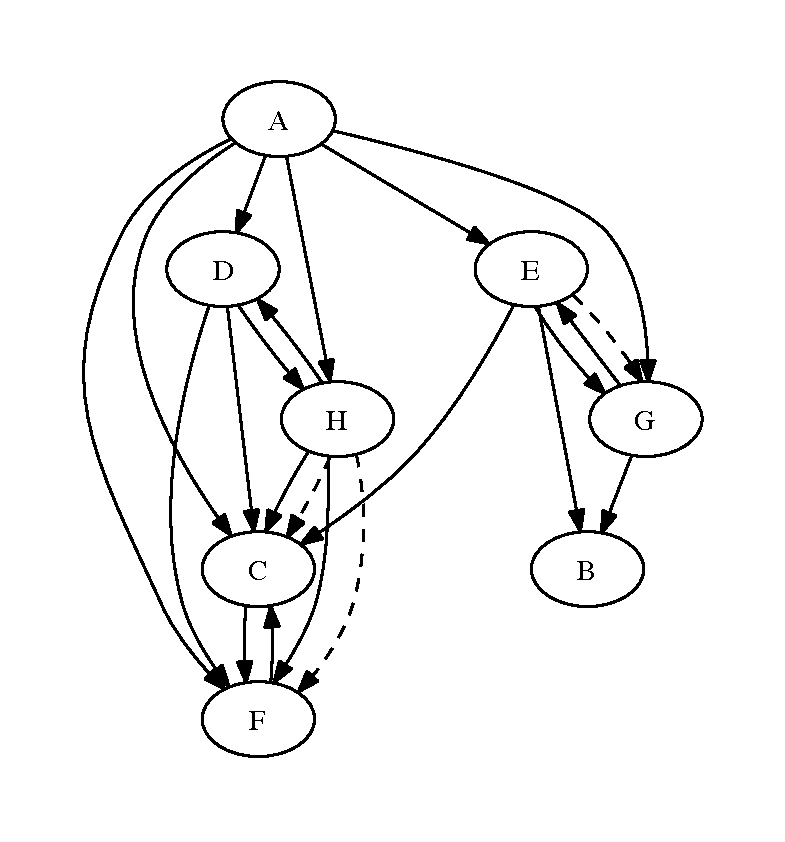
\includegraphics[width=0.5\textwidth]{../SourcesMatlab/electre3-1.pdf}
\caption{Graphe des surclassement sans prise en compte des poids de chaque critère}
\end{center}
\end{figure}

Sur le graphe généré, on voit clairement que la la meilleur solution serait la
solution A car c'est la seule qui n'est dominé par aucune autre.
On voit également que certaines solutions sont équivalentes puisqu'elles se
dominent entres elles. Les couples de solutions \{D, H\}, \{E, G\} et \{C, F\}
sont des couples de solutions équivalentes.
Les solutions F, C et B sont dominés, elles sont donc les moins intéressantes.

Hormis la solution A qui se démarque, il sera difficile d'établir un classement très juste car beaucoup de solutions sont équivalentes entre elles.

\subsection{Avec pondération}

Les pondérations apportés par la partie 2 sont :
\begin{itemize}
\item[g1] : 1.2
\item[g2] : 1.2
\item[g3] : 0.8
\item[g4] : 0.8
\end{itemize}

\clearpage
	
\begin{figure}[!h]
\begin{center}
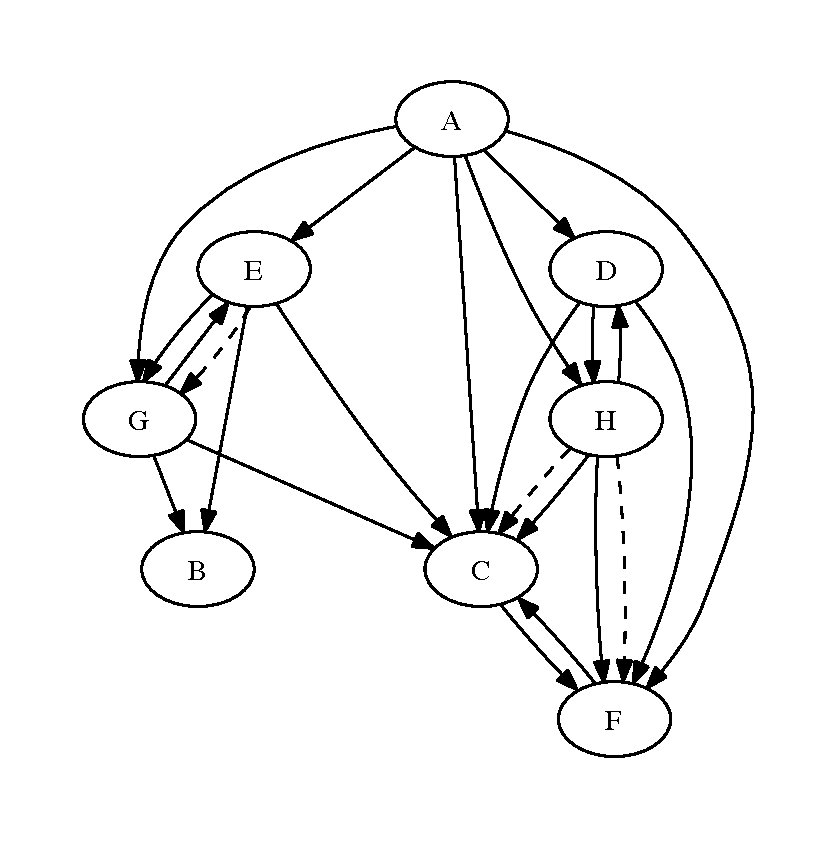
\includegraphics[width=0.5\textwidth]{../SourcesMatlab/electre3-2.pdf}
\caption{Graphe des surclassement avec prise en compte des poids de chaque critère}
\end{center}
\end{figure}

On retrouve la solution A en tête, comme précédemment, et on voit que les positions n'ont pas changé, les surclassement sont presque identiques, seul un surclassement de G sur C est apparu.

\section{Conclusion}

La méthode d'Électre \Rmnum{3} permet de classer un grand nombre de solution suivant plusieurs critères de manière fiable. En pratique elle permet effectivement de tirer des groupes de solutions optimaux d'un ensemble vaste.
Nous avons en effet réussi à isoler une solution optimale parmis les 8 proposés, mais il à été plus difficile d'établir un classement entre toutes les solutions.

\newpage
\nTitle{Annexe}
\section{Code source}
\vfill
\addCode{../SourcesMatlab/Comptable.m}{matlab}
\vfill
\addCode{../SourcesMatlab/Atelier.m}{matlab}
\vfill


\graphicspath{{../SourcesMatlab/}}
\graphicspath{{.}}

\end{document}
